%%%%%%%%%%%%%%%%%%%%%%%%%%%%%%%%%%%%%%%%%
% Beamer Presentation
% LaTeX Template
% Version 1.0 (10/11/12)
%
% This template has been downloaded from:
% http://www.LaTeXTemplates.com
%
% License:
% CC BY-NC-SA 3.0 (http://creativecommons.org/licenses/by-nc-sa/3.0/)
%
%%%%%%%%%%%%%%%%%%%%%%%%%%%%%%%%%%%%%%%%%

%----------------------------------------------------------------------------------------
%	PACKAGES AND THEMES
%----------------------------------------------------------------------------------------

\documentclass{beamer}

\mode<presentation> {

% The Beamer class comes with a number of default slide themes
% which change the colors and layouts of slides. Below this is a list
% of all the themes, uncomment each in turn to see what they look like.

%\usetheme{default}
%\usetheme{AnnArbor}
%\usetheme{Antibes}
%\usetheme{Bergen}
%\usetheme{Berkeley}
%\usetheme{Berlin}
%\usetheme{Boadilla}
%\usetheme{CambridgeUS}
%\usetheme{Copenhagen}
%\usetheme{Darmstadt}
%\usetheme{Dresden}
%\usetheme{Frankfurt}
%\usetheme{Goettingen}
%\usetheme{Hannover}
%\usetheme{Ilmenau}
%\usetheme{JuanLesPins}
%\usetheme{Luebeck}
\usetheme{Madrid}
%\usetheme{Malmoe}
%\usetheme{Marburg}
%\usetheme{Montpellier}
%\usetheme{PaloAlto}
%\usetheme{Pittsburgh}
%\usetheme{Rochester}
%\usetheme{Singapore}
%\usetheme{Szeged}
%\usetheme{Warsaw}

% As well as themes, the Beamer class has a number of color themes
% for any slide theme. Uncomment each of these in turn to see how it
% changes the colors of your current slide theme.

%\usecolortheme{albatross}
%\usecolortheme{beaver}
%\usecolortheme{beetle}
%\usecolortheme{crane}
%\usecolortheme{dolphin}
%\usecolortheme{dove}
%\usecolortheme{fly}
%\usecolortheme{lily}
%\usecolortheme{orchid}
%\usecolortheme{rose}
%\usecolortheme{seagull}
%\usecolortheme{seahorse}
%\usecolortheme{whale}
%\usecolortheme{wolverine}

%\setbeamertemplate{footline} % To remove the footer line in all slides uncomment this line
%\setbeamertemplate{footline}[page number] % To replace the footer line in all slides with a simple slide count uncomment this line

%\setbeamertemplate{navigation symbols}{} % To remove the navigation symbols from the bottom of all slides uncomment this line
}

\usepackage{graphicx} % Allows including images
\usepackage{booktabs} % Allows the use of \toprule, \midrule and \bottomrule in tables
\usepackage{amsmath}
\usepackage{xcolor}
%----------------------------------------------------------------------------------------
%	TITLE PAGE
%----------------------------------------------------------------------------------------

\title[Solving Linear Systems]{Numerical Linear Algebra Workshop} % The short title appears at the bottom of every slide, the full title is only on the title page

\author{Duo Cao} % Your name
\institute[Purdue] % Your institution as it will appear on the bottom of every slide, may be shorthand to save space
{
Department of Mathematics, Purdue University \\ % Your institution for the title page
\medskip
\textit{cao157@purdue.edu} % Your email address
}
\date{\today} % Date, can be changed to a custom date

\begin{document}

\begin{frame}
\titlepage % Print the title page as the first slide
\end{frame}

\begin{frame}
\frametitle{Overview} % Table of contents slide, comment this block out to remove it
\tableofcontents % Throughout your presentation, if you choose to use \section{} and \subsection{} commands, these will automatically be printed on this slide as an overview of your presentation
\end{frame}

%----------------------------------------------------------------------------------------
%	PRESENTATION SLIDES
%----------------------------------------------------------------------------------------

%------------------------------------------------
\section{Background and PDE formulation} % Sections can be created in order to organize your presentation into discrete blocks, all sections and subsections are automatically printed in the table of contents as an overview of the talk
%------------------------------------------------

\subsection{Diffusion Equation}

\begin{frame}
\frametitle{Diffusion Equations}
Diffusive Transport: Dye in water, pollution, heat, perfume...
\begin{figure}
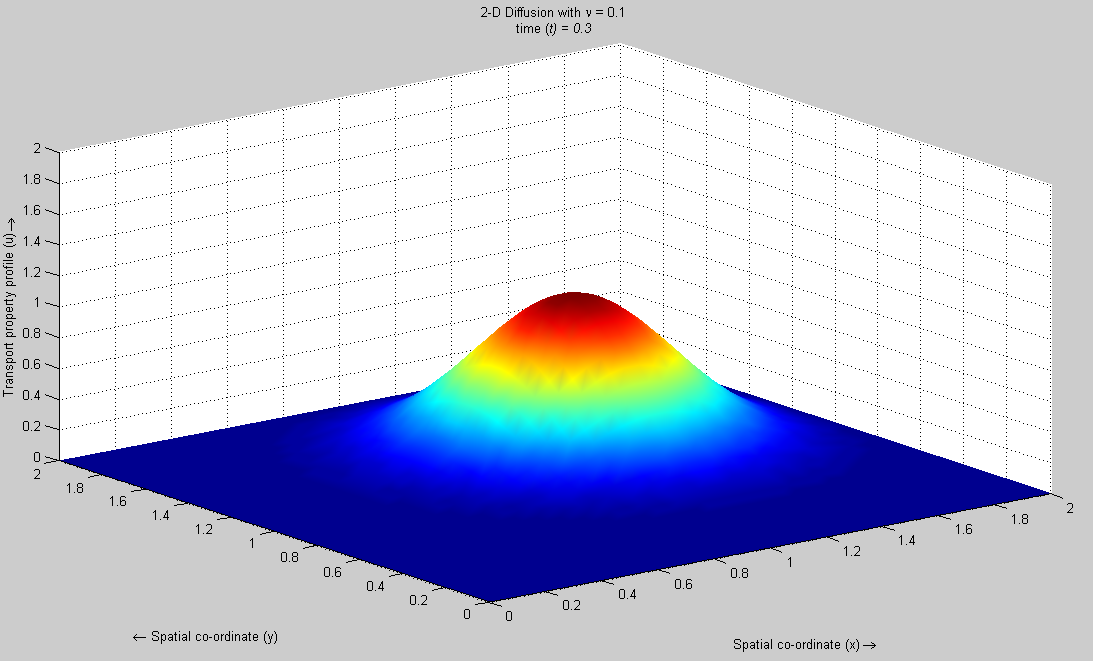
\includegraphics[width=0.8\linewidth]{heat.png}
\end{figure}

\end{frame}

\begin{frame}
\frametitle{Diffusion Equations Cont'd}
\begin{itemize}
\item Consider temperature in a long thin tube of constant cross section.
\item The tube is perfectly insulated laterally. Heat only flow along the tube.
\item Its ends maintain at zero temperature.
\end{itemize}
\begin{figure}
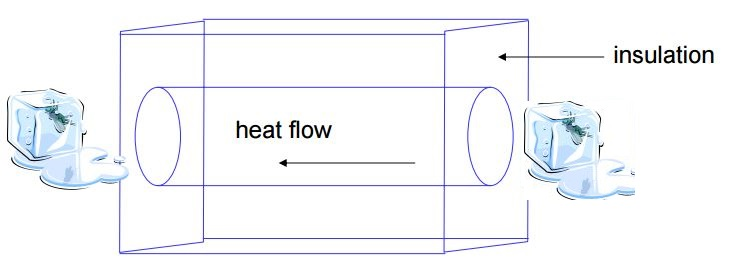
\includegraphics[width=0.6\linewidth]{heat2.jpg}
\end{figure}
\end{frame}

\begin{frame}
\frametitle{Diffusion Equations Cont'd}
\begin{figure}
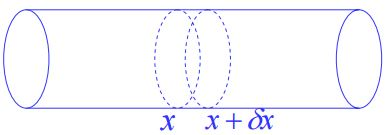
\includegraphics[width=0.4\linewidth]{heat3.jpg}
\end{figure}
Suppose
\begin{itemize}
\item thermal conductivity in the wire is $K$.
\item Cross sectional area is $A$.
\item Material density $\rho$.
\item Heat capacity is $\sigma$.
\item Temperature at point $x$ at time $t$ is $u(x,t)$.
\end{itemize}
Then the heat flow into bar across face at $x: -KA\frac{\partial u}{\partial x}|_x$.\\
At the face $x+\delta x$: $-KA\frac{\partial u}{\partial x}|_{x+\delta x}$
\end{frame}

\begin{frame}
\frametitle{Diffusion Equations Cont'd}
\begin{figure}
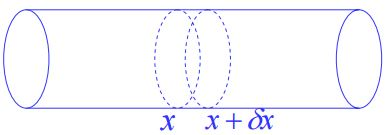
\includegraphics[width=0.4\linewidth]{heat3.jpg}
\end{figure}
\begin{itemize}
\item The net flow out is: $KA\frac{\partial^2 u}{\partial x^2}\delta x$\\
\item $Q = \sigma m \Delta T$\\
\item So, the conservation of heat gives: $KA\frac{\partial^2 u}{\partial x^2}\delta x=\sigma \rho A \frac{\partial u}{\partial t}\delta x$
\end{itemize}
$$\boxed{\frac{\partial u}{\partial t}=c^2\frac{\partial^2 u}{\partial x^2}}$$
\end{frame}

\begin{frame}
\frametitle{Boundary Conditions}
\begin{itemize}
\item Homogeneous Dirichlet Boundary Condition: $u(0,t)=u(L,t)=0$

\item Homogeneous Neumann Boundary Condition: $\frac{\partial u}{\partial x}(0,t)=\frac{\partial u}{\partial x}(L,t)=0$
\end{itemize}
\end{frame}
\subsection{Miscellaneous Equations}
\begin{frame}
\frametitle{Miscellaneous Equations}
\begin{itemize}
\item Navier-Stokes Equation: ${\partial{\bf u}\over{\partial t}} + ({\bf u} \cdot \nabla) {\bf u} = - {1\over\rho} \nabla p + \gamma\nabla^2{\bf u} + {1\over\rho}{\bf F}$
\item Fisher's Equation: $\frac{\partial u}{\partial t}= u(1-u)+\frac{\partial^2 u}{\partial x^2}$
\item Nonlinear Schrodinger Equation: $ i\partial_t\phi=-\frac{1}{2}\partial_x^2\phi+\kappa|\phi|^2\phi$
\item Black-Scholes Equation: $\frac{\partial V}{\partial t}
+ \frac{\sigma^2 S^2}{2} \frac{\partial^2 V}{\partial S^2}
+ r S \frac{\partial V}{\partial S} - rV = 0$
\item etc
\end{itemize}
\end{frame}

%------------------------------------------------
\section{Numerical methods for solving PDEs}
\subsection{Finite Difference Method}
\begin{frame}
\frametitle{Finite Difference Method}
We consider the two-point boundary value problem:
\begin{eqnarray}
Au:&&=-au''+bu'+cu=f \ in \Omega=(0,1),\\
\label{FD}
&&u(0)=u_0,\ u(1)=u_1
\end{eqnarray}

where the coefficients $a=a(x),b=b(x),$and $c=c(x)$ are smooth functions satisfying $a(x)>0$ and $c(x)\geq0$ in\ $\overline{\Omega}$. And $f, u_0, u_1$ are given.
\end{frame}

\begin{frame}
To find numerical solution of (\ref{FD}) we introduce $M+1$ grid points $0=x_0<x_1<...<x_M=1$ by setting $x_j=jh, j=0,...,M$, where $h=1/M$. We denote the approximation of $u(x_j)$ by $U_j$ and use the following finite difference approximation for derivatives.
\begin{eqnarray*}
\partial U_j &=& \frac{U_{j+1}-U_j}{h}, (forward\ difference)\\
\partial \overline{U_j} &=& \frac{U_{j}-U_{j-1}}{h}, (backward\ difference)\\
\widehat{\partial} U_j &=& \frac{U_{j+1}-U_{j-1}}{2h}, (central\ difference)\\
\partial\overline{\partial} U_j &=& \frac{U_{j+1}-2U_j+U_{j-1}}{h^2}
\end{eqnarray*}
\end{frame}

\begin{frame}
Setting also $a_j=a(x_j), b_j=b(x_j), c_j=c(x_j), f_j=f(x_j)$, we now define a finite difference approximation of (\ref{FD}) by
\begin{eqnarray}
A_hU_j&:=& -a_j\partial\overline{\partial} U_j + b_j\widehat{\partial} U_j + c_jU_j=f_j, for\ j= 1, \ldots, M-1,\\
\label{FDSystem}
&&U_0 =u_0,\ U_M = u_1.
\end{eqnarray}
Then, after simplification, the equation at the interior point $x_j$ may be written as
\begin{equation}
(2a_j+h^2c_j)U_j-(a_j-\frac{1}{2}hb_j)U_{j+1}-(a_+\frac{1}{2}hb_j)U_{j-1}=h^2f_j
\label{FDu}
\end{equation}
for all $j$.
\end{frame}

\begin{frame}
Put (\ref{FDu})into a matrix form:
$$\fcolorbox{red}{white}{\textcolor{black}{$AU=g$}} $$
We finally comes to LINEAR ALGEBRA!! OH YEAH!!
\end{frame}

\begin{frame}
In our system $AU=g$:\\
$U = (U_1,\ldots, U_{M-1})^T$ and the first and last components of the
vector $g = (g_1,\ldots, g_{M-1})^T$ contain contributions from the boundary values
$u_0, u_1$ as well as $f_1$ and $f_{M-1}$, respectively. The $(M-1)\times(M-1)$ matrix $A$
is tridiagonal and diagonally dominant for $h$ sufficiently small.
\end{frame}
\subsection{Finite Element Method}
\begin{frame}
\frametitle{Finite Element Method for BVP}
We consider the special case $b=0$ of the two-point boundary value problem of (\ref{FD}),
$$Au:=-(au')'+cu=f \ in\ \Omega:=(0,1),\ with u(0)=u(1)=0,$$
where $a=a(x), c=c(x)$ are smooth functions with $a(x)\geq q_0>0$, $c(x)\geq 0$ in $\overline{\Omega}$ and $f\in L_2 = L_2(\Omega).$
\end{frame}
\begin{frame}
Recall the variational formulation of this problem is to find $u\in H_0^1$ such that
$$a(u,\phi) = (f,\phi), \ \forall\phi \in H_0^1,\label{fem}$$
where
$$ a(v,w) = \int_{\Omega}(av'w'+cvw)dx \ and\ (f,v) = \int_{\Omega}fv dx,$$
and that this problem has a unique solution $u\in H^2$.
\end{frame}
\begin{frame}
For the purpose of finding an approximate solution of (\ref{fem}) we introduce a partition of $\Omega$,
$$0=x_0<x_1<\ldots<x_M=1,$$
and set
$$h_j = x_j-x_{j-1}, K_j = [x_{j-1},x_j],\ for\ j = 1, \ldots , M,\ and\ h=\underset{j}{\max}\ h_j.$$
\end{frame}
\begin{frame}
The discrete solution will be sought in the finite-dimensional space of functions
$$S_h={v\in C=C(\overline{\Omega}): v\ linear\ on\ each\ K_j, v(0)=v(1)=0}.$$
The set $\{\Phi_i\}_{i=1}^{M-1}\subset S_h$ is defined by
\[
\Phi_i(x_j)=
\begin{cases}
1 & if\ i=j \\
0 & if\ i\neq j
\end{cases}
\] 
and any $v\in S_h$ may be written as
$$v(x)=\sum^{M-1}_{i=1}v_i\Phi_i(x),\ with\ v_i=v(x_i).$$
\end{frame}
\begin{frame}
Now we pose the finite-dimensional problem to find $u_h\in S_h$ such that
\begin{equation}
a(u_h,\chi)=(f,\chi),\ \forall \chi \in S_h.
\label{femSys}
\end{equation}
In terms of the basis $\{\Phi_i\}_{i=1}^{M-1}$ we write $u_h(x)=\sum_{j-1}^{M-1}U_j\Phi_j(x)$ and insert this into (\ref{femSys}) to find that this equation is equivalent to 
$$\sum^{M-1}_{j=1}U_ja(\Phi_j,\Phi_i)=(f,\Phi_i), \ for\ i=1,\ldots, M-1.$$
This linear system of equations could be expressed in matrix form as
$$\fcolorbox{red}{white}{\textcolor{black}{$AU=b$}} $$
Finished!!!
\end{frame}
\begin{frame}
In our system $U=(U_j), A=(a_{ij})$ is the stiffness matrix with elements $a_{ij}= a(\Phi_j,\Phi_i)$, and $ b = (b_i)$ with elements $ b_i = (f,\Phi_i)$. The matrix $A$ is symmetric and positive definite, because for $V = (V_i)$ and $v(x)=\sum_{i=1}^{M-1}V_i\Phi_i(x)$ we have
$$V^TAV=\sum_{i,j=1}^{M-1}V_ia_{ij}V_j=a\big(\sum_{j=1}^{M-1}V_j\Phi_j,\sum_{i=1}^{M-1}V_i\Phi_i)=a(v,v)\geq a_0||v'||^2,$$
and hence $V^TAV=0$ implies $v'=0$, so that $v$ is $0$. Matrix $A$ is tridiagonal since$a_{ij}=0$ when $x_i$ and $x_j$ are not neighbors, i.e., when $|i-j|\geq 2$.
\end{frame}
\subsection{Miscellaneous Numerical Methods}
\begin{frame}
\begin{itemize}
\frametitle{Miscellaneous Numerical Methods}
\item{Finite Volume Method}
\item{Spectral Method}
\item{Meshfree Methods}
\item{Multigrid}
\item{etc.}
\end{itemize}
$$\fcolorbox{red}{white}{\textcolor{black}{$AU=b$}} $$
\end{frame}

\begin{frame}


\end{frame}
\begin{frame}


\end{frame}
\begin{frame}


\end{frame}
\begin{frame}


\end{frame}

\begin{frame}
\frametitle{Blocks of Highlighted Text}
\begin{block}{Block 1}
Lorem ipsum dolor sit amet, consectetur adipiscing elit. Integer lectus nisl, ultricies in feugiat rutrum, porttitor sit amet augue. Aliquam ut tortor mauris. Sed volutpat ante purus, quis accumsan dolor.
\end{block}

\begin{block}{Block 2}
Pellentesque sed tellus purus. Class aptent taciti sociosqu ad litora torquent per conubia nostra, per inceptos himenaeos. Vestibulum quis magna at risus dictum tempor eu vitae velit.
\end{block}

\begin{block}{Block 3}
Suspendisse tincidunt sagittis gravida. Curabitur condimentum, enim sed venenatis rutrum, ipsum neque consectetur orci, sed blandit justo nisi ac lacus.
\end{block}
\end{frame}

%------------------------------------------------

\begin{frame}
\frametitle{Multiple Columns}
\begin{columns}[c] % The "c" option specifies centered vertical alignment while the "t" option is used for top vertical alignment

\column{.45\textwidth} % Left column and width
\textbf{Heading}
\begin{enumerate}
\item Statement
\item Explanation
\item Example
\end{enumerate}

\column{.5\textwidth} % Right column and width
Lorem ipsum dolor sit amet, consectetur adipiscing elit. Integer lectus nisl, ultricies in feugiat rutrum, porttitor sit amet augue. Aliquam ut tortor mauris. Sed volutpat ante purus, quis accumsan dolor.

\end{columns}
\end{frame}

%------------------------------------------------
\section{Numerical Method for solving PDEs}
%------------------------------------------------


%------------------------------------------------

\begin{frame}
\frametitle{Theorem}
\begin{theorem}[Mass--energy equivalence]
$E = mc^2$
\end{theorem}
\end{frame}

%------------------------------------------------

\begin{frame}[fragile] % Need to use the fragile option when verbatim is used in the slide
\frametitle{Verbatim}
\begin{example}[Theorem Slide Code]
\begin{verbatim}
\begin{frame}
\frametitle{Theorem}
\begin{theorem}[Mass--energy equivalence]
$E = mc^2$
\end{theorem}
\end{frame}\end{verbatim}
\end{example}
\end{frame}

%------------------------------------------------

\begin{frame}
\frametitle{Figure}
Uncomment the code on this slide to include your own image from the same directory as the template .TeX file.
%\begin{figure}
%\includegraphics[width=0.8\linewidth]{test}
%\end{figure}
\end{frame}

%------------------------------------------------
%----------------------------------------------------------------------------------------
\section{Numerical Linear Algebra}
%----------------------------------------------------------------------------------------

\begin{frame}[fragile] % Need to use the fragile option when verbatim is used in the slide
\frametitle{Citation}
An example of the \verb|\cite| command to cite within the presentation:\\~

This statement requires citation \cite{p1}.
\end{frame}

%------------------------------------------------

\begin{frame}
\frametitle{References}
\footnotesize{
\begin{thebibliography}{99} % Beamer does not support BibTeX so references must be inserted manually as below
\bibitem[Erwin Kreyszig, 2014]{p1}
\newblock Erwin Kreyszig, Advanced Engineering Mathematics, 8th Edn, Sections 11.4b
\end{thebibliography}
}
\end{frame}


%------------------------------------------------

\begin{frame}
\Huge{\centerline{The End}}
\end{frame}


\end{document} 